\begin{figure}[H]
\centering
\begin{subfigure}[b]{0.48\linewidth}
  \centering
  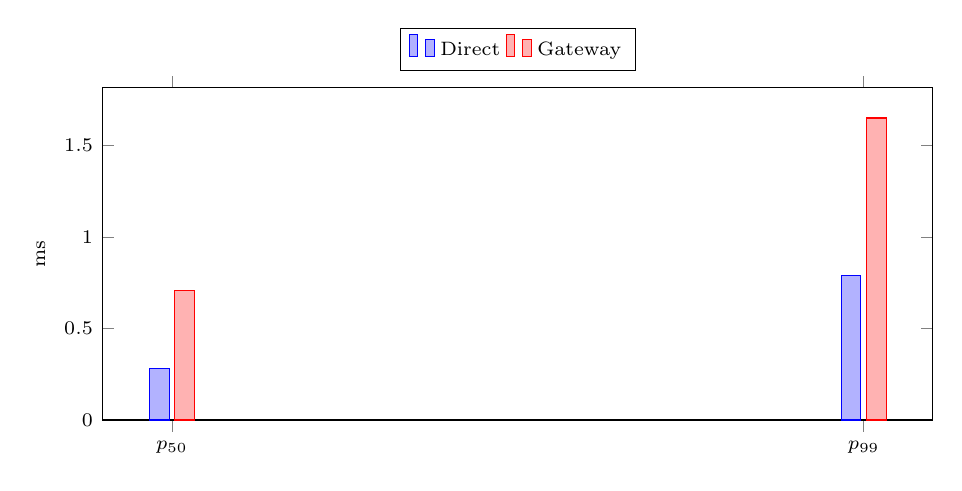
\begin{tikzpicture}
    \begin{axis}[
      width=\linewidth,
      height=5.8cm,
      ybar,
      bar width=0.25cm,
      ymin=0,
      symbolic x coords={$p_{50}$,$p_{99}$},
      xtick=data,
      ylabel={ms},
      legend style={font=\scriptsize,at={(0.5,1.05)},anchor=south,legend columns=2},
      tick label style={font=\scriptsize},
      label style={font=\scriptsize},
    ]
    \addplot coordinates {($p_{50}$,0.28) ($p_{99}$,0.79)};
    \addplot coordinates {($p_{50}$,0.71) ($p_{99}$,1.65)};
    \legend{Direct,Gateway}
    \end{axis}
  \end{tikzpicture}
  \caption{Latency percentiles}
  \label{fig:lat-bars}
\end{subfigure}
\hfill
\begin{subfigure}[b]{0.48\linewidth}
  \centering
  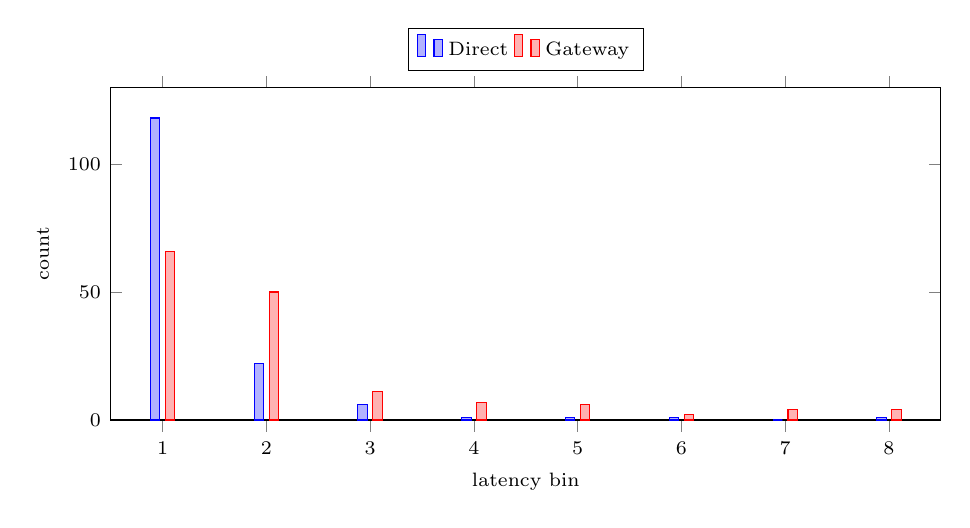
\begin{tikzpicture}
    \begin{axis}[
      width=\linewidth,
      height=5.8cm,
      ybar,
      bar width=0.12cm,
      ymin=0,
      xmax=8.5, xmin=0.5,
      xlabel={latency bin},
      ylabel={count},
      legend style={font=\scriptsize,at={(0.5,1.05)},anchor=south,legend columns=2},
      tick label style={font=\scriptsize},
      label style={font=\scriptsize},
    ]
    \addplot coordinates {(1,118) (2,22) (3,6) (4,1) (5,1) (6,1) (7,0) (8,1)};
    \addplot coordinates {(1,66) (2,50) (3,11) (4,7) (5,6) (6,2) (7,4) (8,4)};
    \legend{Direct,Gateway}
    \end{axis}
  \end{tikzpicture}
  \caption{Latency distribution ($n{=}150$)}
  \label{fig:lat-hist}
\end{subfigure}

\vspace{0.4em}

\begin{subfigure}[b]{0.48\linewidth}
  \centering
  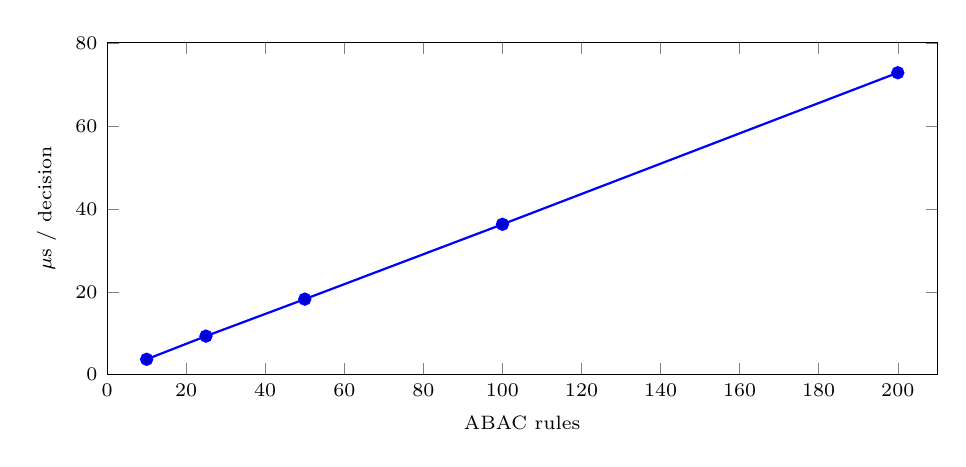
\begin{tikzpicture}
    \begin{axis}[
      width=\linewidth,
      height=5.8cm,
      xmin=0, xmax=210,
      ymin=0,
      xlabel={ABAC rules},
      ylabel={$\mu$s / decision},
      tick label style={font=\scriptsize},
      label style={font=\scriptsize},
    ]
    \addplot+[mark=*,thick] coordinates {(10,3.72) (25,9.31) (50,18.23) (100,36.29) (200,72.86)};
    \end{axis}
  \end{tikzpicture}
  \caption{Policy evaluation cost}
  \label{fig:policy}
\end{subfigure}
\hfill
\begin{subfigure}[b]{0.48\linewidth}
  \centering
  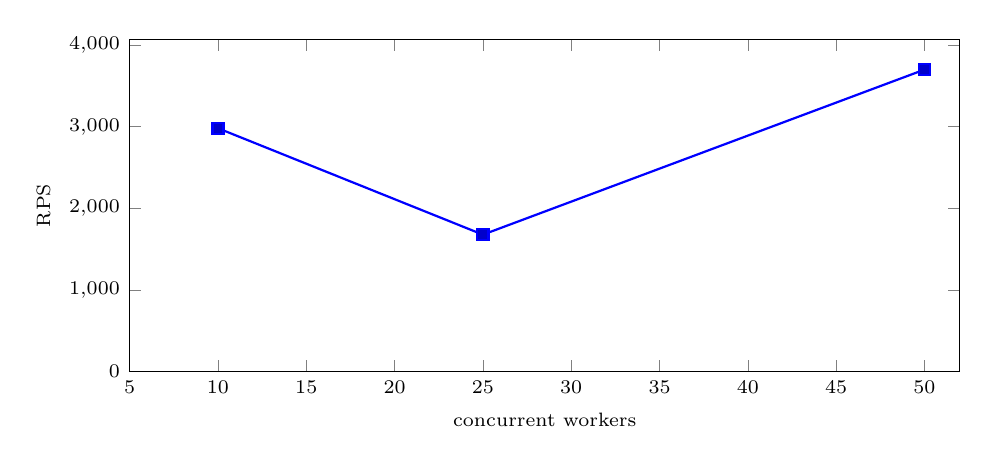
\begin{tikzpicture}
    \begin{axis}[
      width=\linewidth,
      height=5.8cm,
      xmin=5, xmax=52,
      ymin=0,
      xlabel={concurrent workers},
      ylabel={RPS},
      tick label style={font=\scriptsize},
      label style={font=\scriptsize},
    ]
    \addplot+[mark=square*,thick] coordinates {(10,2981) (25,1677) (50,3699)};
    \end{axis}
  \end{tikzpicture}
  \caption{Throughput (\code{tools/call})}
  \label{fig:rps}
\end{subfigure}
\caption{Evaluation on the open research testbed (loopback). Panels (c) and (d) use 50k to 100k policy iterations and a 10\,s load window at 50 workers.}
\label{fig:bench}
\end{figure}
